\chapter{支持动态更新的并发Cuckoo过滤器设计}
%引子
% 对于海量数据处理业务,通常需要建立索引数据结构来帮助查询,快速判断数据记录是否存在,过滤器(filter)能够很好的满足构建索引数据结构的要求。
查找或判断一个元素是否存在于一个指定集合中,这是计算机科学中一个基本问题。
通常会采用线性表(数组或链表)、树(二叉树、堆、红黑树、 B+/B-/B*树)等数据结构存储所有元素,对数据进行排序和查找。
这里的查找时间复杂性通常都是O(N)或O(log(N))。
如果集合元素非常庞大,不仅降低了查找的效率,同时对内存空间的需求也非常大。

在网络安全领域有一个简单的应用场景:判断URL是否链接到存在安全隐患的网站。
用户在浏览器内输入URL,浏览器需要判断该URL是否是恶意的,它将该URL与本地缓存的URL进行匹配,如果匹配失败,则说明该URL是安全的链接可以正常访问;否则,说明该URL可能存在安全隐患。
此时,提交请求给远程客户端进行验证,并警告用户该URL存在风险。
在这个应用场景中,如果缓存的URL数量很少,那么使用上述的数据结构都可以达到较高的查找效率,同时对内存空间的要求也不高。
假设现在需要缓存的URL的数量为10亿条(这在当前是很常见的一个数量级),每条URL的大小为8个字节,那么存储所有的URL大约需要8 GB的内存。
使用哈希表是一种可能的解决方案.哈希表的查询时间复杂度为O(1),可以节省查找的时间,但是没有降低对内存的需求。

事实上,除非有特别的需求,否者判断元素是否在一个指定集合内,并不需要把所有元素的原始信息都保存下来,而只需要保存该元素的“存在状态”,存储存在状态只需要几个bit。
使用哈希函数可以将元素映射成位数组中的一个点,采用k个哈希函数将元素映射成k个点。
这样,经过映射之后,查找元素是否存在时只需看看特定的几个位点的值就能判断某个元素是否存在于集合当中,如果k个位置都为1,则说明该元素可能存在,如果有1个位置上为0,则可以肯定该元素不存在。
这样不仅可大大缩减内存空间,查找速度非常
这就是布隆过滤器(Bloom Filter)的基本思想。
它的名字源自其发明者Burton.H Bloom\cite{bloom1970space}。
布隆过滤器最初应用于拼写检查和数据库系统。
但是,随着互联网的爆炸式发展,海量数据中快速检索目标数据的需求使得布隆过滤器的应用焕发新生,涌现出新的应用和变种\cite{bender2012don,bonomi2006improved,song2005fast,yu2009buffalo}。

\section{布隆过滤器}

\subsection{基本原理}
布隆过滤器使用位数组表示元素集合S,并使用k个哈希函数(h$_1$, h$_2$, ..., h$_k$)来对元素进行位映射。
初始状态下的布隆过滤器是一个包含m位的位数组,每一位都置0,图~\ref{fig:bf}(a)所示为m = 12的布隆过滤器。
当需要将集合S中的n个元素x$_1$,x$_2$, ... x$_n$用位数组表示时,对该元素分别使用k个相互独立哈希函数进行计算,得到位数组上k个位置的索引值,随后将映射到位数组的相应位置1。
值得注意的是,如果一个位置被多次置为1,只有第一次的置位是有效的。
图~\ref{fig:bf}(b)表示k = 3时,将元素映射到位数组的过程,其中元素x$_1$和x$_2$都对第5位置位。
图~\ref{fig:bf}(c)表示判断元素y$_i$(i = 1,2, ..., n)是否属于集合。
与插入过程类似,同样先对y进行k次哈希,如果计算得到的索引值对应的位上有任何一位为0则表示y元素绝对不存在于集合中,只有当所有映射位均为1时才表示该元素\textbf{有可能}存在于集合当中。
\begin{figure}[htbp]
\centering
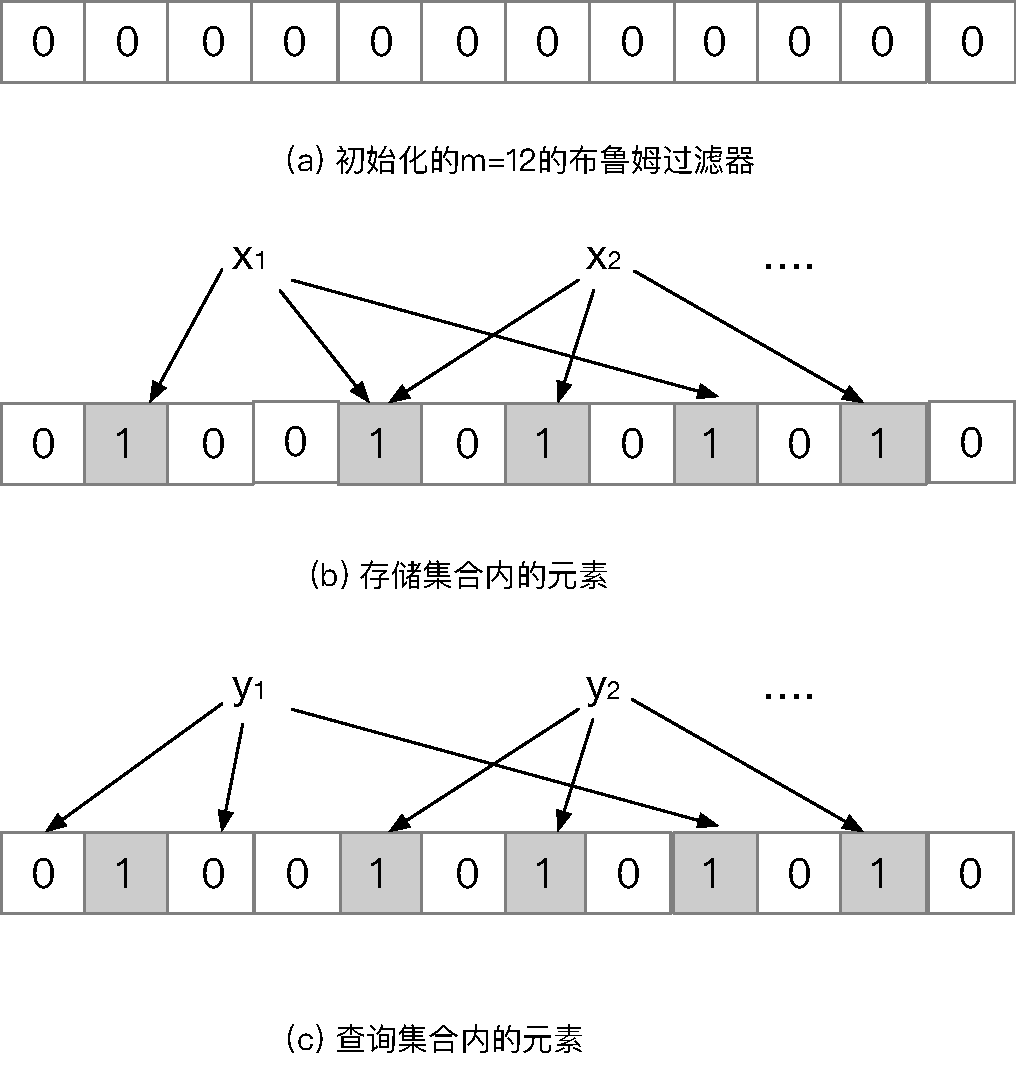
\includegraphics[width=0.65\textwidth]{bloomfilter}
\caption{布隆过滤器}\label{fig:bf}
\end{figure}
换句话说,如果布隆过滤器判断一个元素不在集合中,那肯定就不存在;而如果判断存在,则不一定存在,下文将对这种不一定存在的原因进行说明。
这种不能确定元素一定存在的问题是由哈希函数可能发生碰撞的特性所决定的。
这个错误率可调整位数组大小或者哈希函数个数进行控制。
由此可见,布隆过滤器的高效是以一定的误报为代价的,它通过容忍一定的错误发生的概率换取存储空间的极大节省。
布隆过滤器不适合那些“零错误”的应用场合。

标准的布隆过滤器不支持删除操作。
原因很简单,考虑在图~\ref{fig:bf}(b)中删除元素x$_2$,意味着将位数组内的第5、7、11位置0,此时如果查询x$_1$会发现也不存在,因为它对应的第5位上的值在删除x$_2$时被置0了。

标准布隆过滤器的实现中有几个重要参数:误判率\begin{math}\epsilon\end{math}、负载因子\begin{math}\alpha\end{math}、哈希函数的个数k、位数组大小m和集合中元素的个数n。下面将对这些参数进行推导,以确定实现标准布隆过滤器的参数选取原则。

\subsection{误判率估计}
在进行正式的误判率估计前先明确几个定义和重要的参数:
\begin{definition}
	假阳性(false positives)也叫误判是指当前元素不在集合内,但由于哈希冲突的缘故存在其它元素被映射到部分相同bit位上,从而有一定的概率导致在判定该元素时认定其对应的所有位置都为1,从而判定其在集合内,造成一次误判。这个概率本文称为误判率,误判率用\begin{math}\epsilon\end{math}表示。
\end{definition}

\begin{definition}
	假阴性(false negatives),也叫漏报,是指在位数组内删除某个元素,导致该元素对应的比特位置0,造成本来存在的元素会被漏报成不存在。
\end{definition}

\begin{definition}
	负载因子是指集合中的元素的个数\textit{n},布隆过滤器位数组的位数\textit{m}之间的比值,它用\begin{math} \alpha \end{math}表示,其中\begin{math} \alpha  = {n/m} \end{math}。当\begin{math} \alpha \end{math}为0时,表示布隆过滤器为空,\begin{math} \alpha \end{math}为1表示布隆过滤器满载。
\end{definition}

下面进行误判率\begin{math}\epsilon\end{math}的推算.
首先假设布隆过滤器中使用的k个哈希函数的计算结果都是均匀分布的,即每个元素都等概率地被哈希到m个bit位上的任何一个,与其他元素被哈希到的位置无关。
则对某一特定bit位在一个元素由特定哈希函数插入时没有被置位为1的概率p$_1$为:
\begin{equation}
p_1 = 1-{1/m}
\end{equation}
则k个哈希函数中都没有一个对其置位的概率p$_2$:
\begin{equation}
p_2 = {p_1}^k
\end{equation}
如果插入n(\begin{math}n\leqslant m\end{math})个元素,但都未对其置位的概率p$_3$:
\begin{equation}
p_3 = {p_2}^n = {p_1}^{kn}
\end{equation}
则此位被置位的概率p$_4$为:
\begin{equation}
p_4 = 1 - \left(1 - {1/m}\right)^{kn}
\label{equ:alpha}
\end{equation}
现在考虑判定阶段,若对应某个判定元素的k个位全部置位为1,则可判定其在集合中。因此将某元素误判的概率为:
\begin{equation}
\epsilon = \left(1 - \left(1 - {1/m}\right)^{kn}\right)^k
\label{equ:epsilon}
\end{equation}


由
\begin{math} \left(1 + x\right)^{{1/x}} \thickapprox e \end{math}
可知,但m很大时,满足
$-{1/m}$ $\to 0$,
可将公式\ref{equ:alpha}转化为:
\begin{equation}
\epsilon = \left(1 - \left(1 - {1/m}\right)^{{-m}\frac{-kn}{m}}\right)^k \thickapprox \left(1 - e^{-\frac{nk}{m}}\right)^k
\label{equ:beta}
\end{equation}
由公式\ref{equ:beta}可以初步断定\begin{math}\epsilon\end{math}与元素的个数n和位数组的长度m决定,增大n或者减小m都会导致\begin{math}\epsilon\end{math}的升高。这种计算方法不严格,因为前面假设哈希函数和散列后值的分布是相互独立的。
但是,这个假设随着m和n的增大误判率更接近真实的误判率。
Mitzenmacher证明无假设情况下的误判率的期望值相同\cite{mitzenmacher2002compressed}。

\subsection{最优哈希函数个数}
\label{sec:num_hashf}
哈希函数的选择对于布隆过滤器的性能以及空间利用率都有至关重要的作用。
对于选取什么样的哈希函数已经在前文中有过介绍,这里不再缀述。
而对于哈希函数的个数,直观的认为越多越好。实际上,哈希函数越多,用于表达集合中每一个元素所需要的位数就越多,这与布隆过滤器用较低的误判率换取空间的高效利用的初衷相悖。那么哈希函数的个数应该满足什么条件才能有最佳性能呢?

下面推导对给定的$\alpha$,k满足什么条件可以使$\epsilon$最小化。

令:
\begin{equation}
f\left(k\right) = \left(1 - e^{-{nk/m}}\right)^k 
\end{equation}

取 b = e$^{n/m}$,得:
\begin{equation}
f\left(k\right) = \left(1 - b^{-k}\right)^k 
\end{equation}

两边取对数得: 
\begin{equation}
lnf\left(k\right) = kln\left(1 - b^{-k}\right)
\end{equation}

函数两边对k求导得:
\begin{equation}
{1/f(k)}\cdot f'(k) = ln(1 - b^{-k}) + k \frac{b^{-k}\cdot lnb}{1 - b^{-k}} 
\label{equ:fk}
\end{equation}

对式~\ref{equ:fk}右边求最值。

令:
\begin{equation}
\begin{split}
\frac{1}{f(k)}\cdot f'(k) = ln(1 - b^{-k}) + k\cdot \frac{b^{-k}\cdot lnb}{1 - b^{-k}} = 0 \\
\Rightarrow (1 - b^{-k}) ln(1 - b^{-k}) = -k\cdot b^{-k}\cdot lnb \\
\Rightarrow 1 - b^{-k} = b^{-k} \\
\Rightarrow e^{-\frac{kn}{m}} = \frac{1}{2}\\
\Rightarrow k = ln2\cdot {m/n} \thickapprox 0.7{m/n}
\end{split}
\end{equation}
因此,对于固定的$\alpha$,当$k = 0.7{m/n}$时具有最低的误判率,此时$\epsilon$等于:
\begin{equation}
(1 - {1/2})^k = 2^{-ln2\cdot\frac{m}{n}} \thickapprox 0.62{m/n}
\end{equation}

\subsection{最优位数组长度}
\label{sec:opt_m}
下面进行给定一定的误判率上限,布隆过滤器至少需要多少位才能表示全集中任意的x个元素的集合。
假设全集中元素的个数为n,最大误判率为$epsilon$。以此为前提展开对位数组大小的推导。

假设$S_n$为全集中任取$n$个元素的集合,$B$是表示$S_n$的位数组。
那么对于集合$S_n$中任意一个元素$x$,在$B$中查询$x$都能得到肯定的结果,即$B$能够接受$x$。
显然,由于布隆过滤器引入允许误判,$B$能够接受的不仅仅是$S_n$中的元素,它还允许最多$\epsilon \cdot(u - n)$个误报。因此,对于一个确定的位数组来说,它能够接受总共$n +\epsilon\cdot(u - n)$个元素。在$n + \epsilon\cdot(u - n)$个元素中,$B$真正表示的只有其中$n$个,所以一个确定的位数组可以表示:
\begin{equation}
\binom{n + \epsilon \cdot(u - n)}{n}
\end{equation}
个集合。$m$位的位数组一共有$2^m$个不同的组合,可以进一步推导$m$位的位数组可以表示:
\begin{equation}
2^m\binom{n + \epsilon *\left(u - n\right)}{n}
\end{equation}
个集合。全集中包含n个元素的子集总共有:
\begin{equation}
\binom{u}{n}
\end{equation}
个。因此,要让布隆过滤器的位数组大小能够满足所有包含n个元素的子集,必须满足:
\begin{equation}
2^m\cdot\binom{n + \epsilon \cdot(u - n)}{n} \geq \binom{u}{n}
\end{equation}
即m需要满足:
\begin{equation}
m \geq log_2({\binom{u}{n}/\binom{n + \epsilon \cdot(u - n)}{n}}) \geq log_2({\binom{u}{n}/\binom{\epsilon u}{n}}) \thickapprox log_2\epsilon^{-n} = n log_2({1/\epsilon})
\label{equ:bfm}
\end{equation}
式~\ref{equ:bfm}中近似相等有个重要的前提条件:$n$远小于$\epsilon\cdot u$,这个前提在实际的问题中也是常见的。
根据式~\ref{equ:bfm}中的不等式,得到如下结论:在误判率上限为$\epsilon$的情况下,$m$至少要等于$nlog_2{1/\epsilon}$才能表示任意$n$个元素的集合。

在本章~\ref{sec:num_hashf}中推导出哈希函数的个数$k$等于$k = 0.7{m/n}$时可以得到最小误判率,此时的误判率为$(\frac{1}{2})^{0.7{m/n}}$。
令$(\frac{1}{2})^{0.7{m/n}} \leq \epsilon $,可以进一步推导:
\begin{equation}
m \geq n\frac{log_2({1/\epsilon})}{ln2} = nlog_2e\ast log_2({1/\epsilon}) \thickapprox 1.44n\cdot log_2({1/\epsilon})
\label{equ:bfm2}
\end{equation}

式~\ref{equ:bfm2}说明当k取到最优值时,要保证误判率不超过给定的上限$\epsilon$,$m$至少要取到最小值的1.44倍。
可以验证,当给定$\epsilon = 0.01$时,存储每个元素需要9.6比特。
而将$\epsilon = 0.001 $时,每个元素需要额外的增加4.8比特。
所以,在实际的应用中,对于误判的容忍度不同,要求误判率越低,则存储每个元素需要的比特位越多,相同容量下存储的元素个数就越少。

\section{Cuckoo过滤器的参数}
\label{sec:cbf_para}
传统的布隆过滤器的空间效率高,对插入和查询元素的处理也相当快。
但是它也存在缺陷——存在一定的误报率,不支持元素的删除操作。
消除误报率除非能实现没有碰撞的哈希函数,但是不发生碰撞的哈希函数至今没有被设计出来。
研究人员能做的就是尽量选择均匀的哈希函数,并且借助一些数据结构的特性有效的对碰撞进行处理。
而在上一节的中介绍到误判率每缩小到原来的十分之一,至少要增加4.8个比特位用于表示一个元素。
另外,实现元素删除操作的一个方法是引入计数器,将每个比特位都扩张成一个计数值,降低了空间效率。
为了支持对元素的删除操作,出现了很多标准布隆过滤器的扩展版本\cite{bender2012don,bonomi2006improved,fan2000summary}。
所以,布隆过滤器实现更低的误判率和实现删除操作都需要牺牲一定的空间效率。

为了解决上述问题,本文引入一种新的数据结构——Cuckoo过滤器。
它既可以确保该元素存在的必然性,即将“可能存在”变成“一定存在”;
又支持动态的对元素的插入和删除,而不会造成漏报。

为了支持动态的插入和删除元素,Cuckoo过滤器采用的是一种称为\textbf{不完整键值(partial-key)} Cuckoo哈希的技术。
Cuckoo过滤器是标准Cuckoo哈希表在集合元素查询算法领域的应用。
在前面的章节中已经对Cuckoo哈希表的基本原理和概念有过详细介绍(\textcolor{red}{第~\ref{sec:XX}节}),这里不再赘述。
仅对与在这一部分密切相关的术语进行重申。
Cuckoo的数据结构与Cuckoo哈希表相同,其基本单元称为\textbf{实体}(entry),不同的是每一个实体内存储的不是完整的键值,而是根据键值进行提取后的\textbf{指纹}(fingerprint)~\cite{memc3},用$f$表示。
哈希表由存储了多个实体的\textbf{桶}(bucket)数组构成。

表~\ref{tab:ckf_para}列出了本小节所用到的一些关键参数及其含义。
\begin{table}[htbp]
  \centering
  \caption{相关符号及其含义}
  \label{tab:ckf_para}
  \begin{tabular}{cc}
    \toprule
      参数  & 含义  \\
    \midrule
      $\epsilon$  					  &   误判率 \\
        f 							  &   指纹信息的长度(单位:bit)\\
      $\alpha$					      &   负载因子($0\leq\alpha\leq 1$) \\
    	b                             &   每个哈希桶内包含的实体的数量 \\
    	m 							  &	  哈希桶的数量 \\
    	n                             &   元素的数量 \\
        C 							  &   表达一个元素所需的平均位数(单位:bit)\\
    \bottomrule
  \end{tabular}
\end{table}

\subsection{指纹信息的长度}
在这一部分中,将探讨构造Cuckoo过滤器的几个关键参数。
在Cuckoo过滤器中使用不完整键Cuckoo哈希方法存储指纹信息会导致指纹信息的下界值随着过滤器大小的增加而缓慢增加。
这与用传统方法实现的过滤器相反,在标准布隆过滤器中,指纹信息的大小只与预定的$\epsilon$有关。这个看上去似乎是Cuckoo过滤器的劣势,实际上它造成的影响微乎其微。

\subsubsection{指纹信息下界约束}
在Cuckoo过滤器中,对于一个给定的元素,根据其当前位置和指纹信息使用不完整键哈希方法可以推导出它的备选哈希桶的索引值。
这样,每个元素的候选哈希桶都不是独立的。
比如,某一元素可以存放在桶$i_1$或$i_2$中,对于长度为$f$比特的指纹信息,根据公式~\ref{equ:ckf},$i_2$可能的索引值最多有$2^f$种可能。
若指纹信息的长度为一个字节,对给定的$i_1$,$i_2$最多只能偏离$i_1$ 256个位置。
对于具有$m$个桶的哈希表而言,当$2^f \leq m$时,$i_2$能够选择的哈希桶的范围只是整个$m$个哈希桶的一个很小的子集。
这会引起更多的碰撞。

直观上看如果指纹信息的长度足够长,不完整Cuckoo哈希仍然能够接近标准Cuckoo哈希的冲突处理能力。
然而,如果哈希表非常大,而此时指纹信息的长度相对来说要远远小于哈希表的大小,这样容易引起更多的哈希碰撞,从而导致插入失败的概率升高。
当Cuckoo过滤器需要处理大量元素,而$\epsilon$设定一个s中等偏低的值时,可能发生上述情形。
接下来,将通过分析确定插入失败的概率下限。

首先推导对于给定的$u$个元素,它们恰好映射到相同的两个哈希桶内的概率$p_1$。
假设第一个元素$x$位于桶$i_1$内,并且指纹为$t_x$。
如果其他的$u-1$个元素具有与$x$相同的桶索引值,它们必然满足以下两个条件:(1)它们的指纹都为$t_x$,出现的概率为$\frac{1}{2^f}$;
(2)它们第一个桶索引值为$i_1$或者$i_1 \bigoplus h(t_x)$,出现的概率为$\frac{2}{m}$。
因此,$u$个元素映射到相同的两个桶内的概率$p_1 = (\frac{2}{m}\ast \frac{1}{2^f})^{u-1}$

现在考虑构建Cuckoo过滤器的随机插入$n$个元素的构建过程。
假设初始化的哈希表桶数组满足$m = cn$,每个哈希桶容纳的元素个数为$b$,其中$c$为常数。
当出现$u = 2b+1$个元素被映射到相同的两个桶内时,插入失败。
这个概率为插入失败的概率下界。
由于从$n$个元素中包含$2b+1$个元素的子集有$\binom{n}{2b+1}$个,$2b+1$个元素在插入过程中发生碰撞的期望值为:
\begin{equation}
\binom{n}{2b+1}(\frac{2}{2^fm})^{2b} = \binom{n}{2b+1}(\frac{2}{2^f{cn}})^{2b} = \Omega(\frac{n}{4^{bf}}) 
\label{equ:cbf_f}
\end{equation}

因此,由式~\ref{equ:ckf_f}可以做出结论,$4^{bf}$必须满足$\Omega(n)$才能避免一场的插入失败的概率。
指纹信息的长度最好为$f = \Omega(log(\frac{n}{b}))$比特。
在第~\ref{sec:opt_m}节中指出标准的布隆过滤器用于表示每个元素所需的比特数为常数(近似等于$ln(\frac{1}{\epsilon})$)。
而Cuckoo过滤器指纹信息所需的长度为$\Omega(logn)$这个级别,这个结果看上去似乎不是特别理想。
这会不会引起扩展性问题呢?
实验表明桶容量$b$的在下界约束中的起决定作用:只要将$b$控制在合理的大小,指纹信息的长度仍然可以保持较小的值。

\subsubsection{实验评估}
%实验评估
图~\ref{fig:cbf_fingerprint_size}所示为负载因子与指纹信息长度$f$,哈希桶容量$b$以及哈希表总的哈希桶数量$m$的数量关系曲线。
$x$轴表示指纹信息的大小($1~\leq ~f~\leq ~20$),$y$轴表示负载因子($0~\leq ~\alpha ~\leq 1$)。
图~\ref{fig:cbf_fingerprint_size}(a)、(b)所示分别为$b = 4,8$时指纹信息长度与负载因子的变化关系。
实验时,插入的键为64位的随机值。
认定哈希表“饱和”的条件是:当执行某次插入操作时,进行了多达500次的替换操作之后仍没有找到空闲的位置接纳被踢出的元素。
当哈希表达到”饱和“之后,停止本次测试并记录此时哈希表的负载因子。
每组参数运行十次,最终结果取十次的平均值。
\begin{figure}[htbp]
\centering
\subfigure[$b$~= ~4 ]{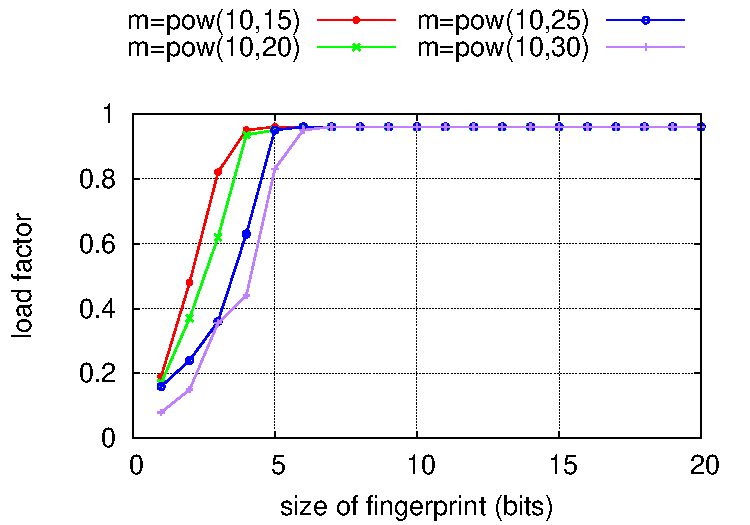
\includegraphics[width=0.45\textwidth]{cbf_loadfactor_b4}}
\subfigure[$b$~ = ~8]{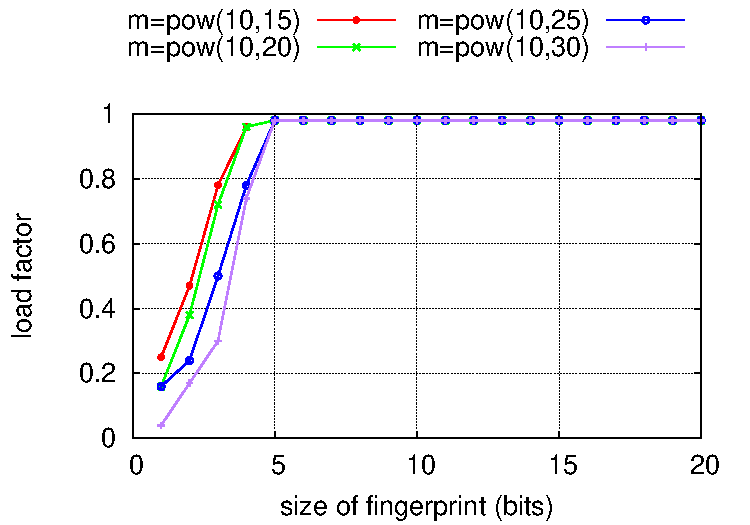
\includegraphics[width=0.45\textwidth]{cbf_loadfactor_b8}}
\caption{负载因子与指纹信息长度变化关系}
\label{fig:cbf_fingerprint_size}
\end{figure}

如图~\ref{fig:cbf_fingerprint_size}所示,在所有的参数组合中,$b = 4$的过滤器的哈希表的利用率能够达到95\%,而$b = 8$的过滤器在指纹信息大小足够长的前提下哈希表利用率可以达到98\%。利用率达到这些值后,增加指纹信息的长度对哈希表利用率的提升几乎没有帮助(但是可以降低误判率)。
通过前文的理论分析表明,当过滤器的规模增大时,所需的$f$的最小值会发生变化。
此外,通过比较图~\ref{fig:cbf_fingerprint_size}(a)和图~\ref{fig:cbf_fingerprint_size}(b)发现达到高哈希表利用率的$f$的最小值随着哈希桶容量$b$的增加而减小,这个规律同样的也与前文的理论推算吻合。
在本次实验中,使用两个完全独立的哈希函数,当$b = 4$且$m = 2^{30}$时,哈希表最多能存储多达40亿个元素,而当指纹信息的长度大于6比特时,$\alpha$接近"最优负载因子"。

\subsubsection{启示}
通过结合公式~\ref{equ:cbf_f}对$f$的下界约束推导的结果与图~\ref{fig:cbf_fingerprint_size}中的实验结果可以总结出Cuckoo过滤器的一条非常重要的结论。
在理论上Cuckoo过滤器的空间效率要比标准布隆过滤器“差”——
$\Omega(log~n)$与常数间的区别。
对于布隆过滤器而言,不论哈希表存储的元素个数是一千、一百万还是数十亿,达到百分之一的误判率大约都只需要10个比特位来表示每个元素。
而为了保持相同的空间效率Cuckoo过滤器需要使用更多的比特位表示每条指纹信息。
同样的由理论推算过程可知,$f$为$\Omega(log~n)$比特,如果$b$足够大,则$f$的值增长非常缓慢,在实际的应用中,可以将其视为常数。
图~\ref{fig:cbf_fingerprint_size}的结果表明6比特的指纹信息足够存储数十亿个元素,并且能够达到很高的哈希表利用率。

\subsection{空间效率}
对Cuckoo过滤器内的元素进行增、删、查操作与每个哈希桶内包含多少实体无关。
但是,为Cuckoo过滤器选择正确的参数对于空间效率具有重要意义。
这一部分着重介绍如何选取合适的参数优化Cuckoo过滤器的空间效率。

\subsubsection{空间开销}
空间效率是通过计算在完整的过滤器中用于表示每个元素所用的平均比特数来衡量的。
用哈希表的大小除以过滤器有效存储的元素的个数就是表示每个元素所用的平均比特数。
尽管每个实体可以存储一条指纹信息,但是并不是所有的实体都已经存入了指纹信息——过滤器的哈希表内一定有空闲的实体。
所以,每个元素实际上需要的比特数大于指纹信息的长度。
如果每条指纹信息的长度为$f$比特,哈希表的负载因子为$\alpha$,则每个元素的空间开销C为:
\begin{equation}
C = \frac{\text{哈希表的大小}}{\text{元素个数}} = \frac{f\cdot \text{实体数量}}{\alpha \cdot \text{实体的数量}} = \frac{f}{\alpha} \text{bits.}
\label{equ:space_cost}
\end{equation}

在前文中有过介绍,指纹信息的长度和负载因子都与哈希桶的大小有关。
下面研究在给定的误判率$\epsilon$前提下,如何通过选取最优的桶大小$b$使$C$最小化。

保持Cuckoo过滤器的总的大小为常量,改变哈希桶的大小会产生两方面的影响:
\begin{itemize}
\item \textbf{哈希桶容纳的实体数量越多,哈希表的空间占用率就越高。}对于使用两个哈希函数的Cuckoo过滤器,当桶能容纳的实体数$b = 1$时,哈希表的负载因子$\alpha$为50\%,
而当$b = 2,4,8$时,$\alpha$分别为84\%,95\%和98\%。
\item \textbf{哈希桶的容量越大,维持相同$\epsilon$需要的指纹信息的长度越长。}
哈希桶的容量越大,进行查询时需要检查更多的实体,并且发现相同指纹信息的概率也会增加。
在最坏情况下,查询一个并不存在的元素需要探测两个分别包含了$b$个实体的桶
(当然并不是所有的哈希桶内都填满了实体,这里只是考虑最糟糕的情况;当哈希表的负载因子达到95\%时,已经很接近极限情况)。
对于每一个实体而言,一次查询与存储的指纹相匹配并且返回成功匹配误报的概率最多为${1/2^f}$。
在进行$2b$次这样的比较之后,误报率的上界为:
\begin{equation}
1 - (1 - {1/2^f})^{2b} \thickapprox {2b/2^f}
\end{equation}
该上界约束与哈希桶的容量$b$成正比。
为了保证预定的误报率$\epsilon$不变,必须确保${2b/2^f}\leq \epsilon$,保证这个条件的最小指纹信息长度为:
\begin{equation}
f \geq \lceil log_2({2b/\epsilon})\rceil = \lceil log_2({1/\epsilon}) + log_2(2b)\rceil  
\label{equ:upper_f}
\end{equation}
\end{itemize}

由式~\ref{equ:space_cost}和\ref{equ:upper_f}可以推算存储每个元素的空间开销$C$受下面条件的限制:
\begin{equation}
C \geq {\lceil log_2({1/\epsilon}) + log_2(2b)\rceil /\alpha}
\label{equ:space_cost_bound}
\end{equation}
$\alpha$随着$b$的增加而增加。
当$b = 4$时,$\alpha = 0.95$,${1/\alpha} \thickapprox 1.05$。
此时$C$ = 1.05$log_2({1/\epsilon}) + 1.05\cdot 3$。
式~\ref{equ:space_cost_bound}表明,当负载因子一定时,Cuckoo过滤器的空间开销要低于布隆过滤器($1.44log_2({1/\epsilon})$)。

\textcolor{red}{为了确定最优的哈希桶容量$b$,下面将通过实验比较参数$b$为不同的值时的空间效率。
用不完整键Cuckoo哈希方法构造具有不同的指纹信息长度的哈希表,分别记录对应的平均空间开销和误判率。
结果如图~\ref{fig:cbf_opt_b}所示。
使空间效率最好的$b$的取值依赖于预定的误判率$\epsilon$:当$\epsilon > 0.002 $时,$b = 2$对应的平均空间开销要略好于$b = 4$对应的空间开销;而当$ 10^{-5} < \epsilon \leq 0.002$时,$b = 4$具有最小的空间开销。}

综上所述,Cuckoo过滤器的默认参数配置为(2,4),即每个元素有两个候选的哈希桶,每个哈希桶最多能够容纳4条指纹信息。
选取这组参数作为默认配置的原因一是实际的应用一般都要求$ 10^{-5} < \epsilon \leq 0.002$~\cite{broder2004network},二是这个参数组合能够提供最优综合性能。

\section{并发Cuckoo过滤器}
无论是标准的布隆过滤器还是现有的其他一些布隆过滤器的扩展版本,都具有在单核平台上快速处理元素的能力以及高效的空间利用率。
单核处理器的计算能力已达到瓶颈,相对而言多核计算机的计算资源和计算能力更加充裕。
在当前数据呈现爆炸式增长的背景下,海量数据处理压力越来越大,单核处理器上的过滤器逐渐显得捉襟见肘。
因此,设计基于多核系统的多线程并发的过滤器对于海量数据处理无疑是雪中送炭。
然而,当前的相关研究中并没有一款支持多核并发查询和更新的过滤器。

并发控制在多核平台上设计并发数据结构的关键环节,它对线程扩展性和整体性能起决定作用。
在前面对并发哈希表的评估与分析中通过比较各个并发哈希表的线程同步方式发现不当使用共享变量以及使用TAS锁不利于并发哈希表的线程扩展性。
本文设计的并发Cuckoo过滤器其基础数据结构本质上仍然是哈希表,不同的是Cuckoo过滤器结合了处理集合成员查询问题的特征改用存储不完整键值替换标准Cuckoo哈希表中存储完整的键值信息的做法,换取存储空间的极大节省。
因此,前文通过实验评估得出的结论仍然适用于并发Cuckoo过滤器。

在这个背景下,设计了一种支持多核并发的基于不完整键Cuckoo哈希方法的过滤器。
这一部分主要介绍并发Cuckoo过滤器的实现过程和性能评估结果。

\subsection{加锁与解锁}
接下来的内容介绍如何通过基于Intel RTM的MCS锁实现多线程并发的Cuckoo过滤器。
Listing 2.1 给出了基于Intel RTM的MCS锁算法实现。
$locklib\_mutex\_t$是一个包含了MCS锁字段、一个$uint8\_t$类型的$mode$变量以及一个用于缓存行对齐的字符串的结构体。
函数$locklib\_mutex\_lock()$具有两个参数,一个为互斥量$mutex$,一个为整型数$mode$。
$mode$的值分别对应0、1,0表示当前持有锁的操作为读取操作,1表示当前持有锁的操作为更新操作(删除或插入)。
\begin{lstlisting}[caption = {基于Intel RTM的MCS锁算法}]
struct {
        mcs_lock_t    lock;
        uint32_t    pad1[128/4 - sizeof(mcs_lock_t)];
} spec_mcs_lock_t;

struct {
        mcs_lock_t        mcs;
        uint8_t mode;
        char padding[];
} locklib_mutex_t;

int locklib_mutex_lock(locklib_mutex_t *mutex, uint8_t mode){
        spec_mcs_lock_t *lock = (spec_mcs_lock_t *) mutex;
        uint32_t reason = 0;

speculative_path:
        XBEGIN(fallback_path, reason);
        if (lock->lock) XABORT(1);
        return 0;

fallback_path:
        retries++;
        while (lock->lock)
                cpu_relax();
        if (retries < MAX_RETRIES)
                goto speculative_path;

        // Acquire lock in a standard manner
        my_node.locked = true;
        qnode_t *prev = __sync_lock_TAS(&lock->lock, &my_node);
        if (unlikely(prev != NULL)) {
                prev->next = &my_node;
                while (my_node.locked)
                        cpu_relax();
        }
        mutex->mode = mode;
        return 0;}
\end{lstlisting}
对临界区的保护设置了$speculative\_path$,$fallback\_path$两条执行路径:一条为事务化推测执行路径(第16行);一条为回退路径(第21行),即当事务执行失败后,临界区申请标准锁完成本次操作。
在事务化推测执行期间,线程首先不会申请获取锁,直到执行完成准备提交时再申请获取锁,如果申请的锁被占用,则该线程所执行的事务被中止,
线程对系统状态所做的更改都失效,系统回退到初始状态跳转到回退路径执行(事务内存的原子性)。

跳转到回退路径之后,如果当前重试的次数没有达到预先设定的门限值,将继续尝试进行事务化推测执行(第23-26行)。
如果当前重试次数已经达到了门限值,则使用标准的锁方法完成操作(第29-35行)。

由于硬件事务内存不能保证每次事务化执行都能成功提交对系统状态的更改,为了避免进程悬停,在使用硬件事务内存进行锁省略编程时设置回退路径是有效的保障程序顺利执行的手段。
一般的,事务代码在经过一定次数的重试之后成功提交的概率远远大于失败的概率,所以执行回退路径对性能的影响是可控的。

% \begin{figure}
\begin{lstlisting}[caption = {基于Intel RTM的MCS解锁算法}]
int locklib_mutex_unlock(locklib_mutex_t *mutex)
{
    spec_mcs_lock_t *lock = (spec_mcs_lock_t *) mutex;

    if (XTEST()) {
        XEND();
    } 
    else {
        // Release lock in a standard manner
        qnode_t *last = my_node.next;
        if (last == NULL) {
            if (likely(true == __sync_bool_CAS
            	(&lock->lock, &my_node, NULL)))
                	return 0;

            while ((last = my_node.next) == NULL)
                	cpu_relax();
            }

        my_node.next = NULL;
        last->locked = false;
    }

    retries = 0;
    return 0;
}
\end{lstlisting}

Listing 2.2 展示了对应的解锁过程。
与加锁过程的两条路径相对应,释放锁的过程也分为两个阶段:首先使用\textit{XTEST}判断当前执行的操作是否为事务执行,若为事务执行,使用\textit{XEND}结束;若判断此次操作申请的锁是通过标准的方式获取的,则按照标准锁的释放过程释放锁。
最后将\textit{retries}变量清零。

\subsubsection{并发访问接口}

\begin{table}[htbp]
  \caption{HashTable类的成员函数列表}
\label{tab:cbf_API}
\footnotesize
\centering
\begin{tabular}{ccc}
\toprule
序号&API &   描述  \\
\midrule
1	&	explicit ~\textbf{HashTable(num)}									 	&  	构造函数\\
2	&	 ~\textbf{HashTable()}  									& 	析构函数\\
3	&	size\_t  \textbf{NumBuckets()} 									&  	返回哈希桶数量\\
4	&	size\_t  \textbf{SizeInBytes() }									&  	返回哈希表大小(单位:Bytes)\\
5	&	size\_t  \textbf{SizeInTags()} 									&  	返回哈希表容纳的指纹的数量\\
6	&	string   \textbf{Info()} 											&  	返回哈希表的容量信息\\
7	&	uint32\_t  \textbf{ReadTags(i, j)}										&  	读取指纹信息\\
8	&	void  \textbf{WriteTags(i, j, t)} 										&  	修改指纹信息\\
9	&	bool  \textbf{ ConFindTagInBuckets(i1, i2, tag) }			& 	并发查找接口\\
10	&	bool  \textbf{ ConDeleteTagFromBucket1(i, tag)	}			& 	并发删除接口\\
11	&	ReturnCode  \textbf{ ConInsertTagToBucket(i, tag, kickout, \&oldtag) }	& 并发插入接口\\
\bottomrule
\end{tabular}
\end{table}

并发Cuckoo过滤器的实现使用了大约500行C++代码。
在这一部分中,将对并发Cuckoo过滤器\textbf{HashTable}类的主要API进行介绍。
表~\ref{tab:cbf_API}~列出了Cuckoo过滤器的\textit{HashTable}类的主要API。
序号3-5对应的API主要用于统计哈希表的信息,用于最终计算哈希表的负载因子,内存消耗等;序号6对应的API输出指纹信息的长度、每个哈希桶能容纳的指纹信息的数量、哈希桶的数量、哈希表的最大指纹容量等信息;序号7、8对应的API分别用于读取和修改指定的指纹信息;序号9-11对应的API实现在哈希表内并发的读取和修改元素。

下面对Cuckoo过滤器的三种元素操作的多线程并发实现进行描述。

\subsection{插入操作}
在标准Cuckoo哈希表中,在哈希表中插入新的元素时需要以某种方式读取原本存储于哈希表内的元素,以便在发生踢出原始元素时确定将该元素安置在哪个位置上。
但是,对于只存储了指纹的Cuckoo过滤器而言,它无法根据原始元素的键计算出旧键迁移到哪个位置。
这里引入不完整键Cuckoo哈希算法来解决无法根据指纹信息定位旧键迁移位置的问题。
对任意的元素\textit{x},使用公式~\ref{equ:ckf}计算其两个备选哈希桶的索引值:
\begin{equation}
\begin{split}
h_1\left(x\right) &= hash\left(x\right) \\
% \label{equ:ckf1}
% \end{equation}
% \begin{equation}
h_2(x) &= h_1(x)\bigoplus hash(\text{x的指纹信息})
\end{split}
\label{equ:ckf}
\end{equation}

式~\ref{equ:ckf}的异或操作有一个重要的特性:$h_1(x)$可以通过$h_2(x)$和指纹信息用同样的公式推算出来。
即就是说,替换编号为$i$的哈希桶中的旧键(不论$i$对应的是$h_1$还是$h_2$),都可以通过当前桶编号\textit{i}以及存储在该桶内的指纹直接计算出旧键的备选哈希桶的编号\textit{j},计算方式为:$j = i \bigoplus hash(\text{指纹信息})$。

因此,在进行插入操作时,不用检索目标哈希桶内存储的元素的完整信息,只需要存储在哈希表中的指纹信息。

另外,为了使众元素在哈希表中均匀分布,在与索引值进行异或运算之前,指纹信息已经进行过哈希运算。
当指纹信息远小于哈希表的大小时,如果直接使用索引值与未经哈希的指纹信息进行异或运算推算接纳被踢出元素的哈希桶的位置,那么接纳被踢出的元素哈希桶与原来的哈希桶在位置上很近。
下面举例说明。
使用8比特的指纹信息时,接纳从\textit{i}中被踢出的元素的哈希桶的位置距离\textit{i}的最大距离为$2^8 = 256$。
这时因为在进行异或运算时,会选取索引值的低8位进行运算,而高8位保持不变。
对指纹信息进行哈希能够确保这些元素尽量分散在哈希表的不同位置,从而可以避免哈希碰撞,提高哈希表的空间利用率。
\SetKwProg{Fn}{Function}{}{}
\begin{algorithm}[htbp]
\SetAlgoLined
\# define UPDATE\_LOCK ~~~ locklib\_mutex\_lock(mutex, 1)\\
\# define UPDATE\_UNLOCK ~~~ locklib\_mutex\_unlock(mutex)\\
\Fn{Insert(x)}{}{
f = fingerprint(x)\\
i1 = hash(x)\\
i2 = i1~$~~\bigoplus~~$~hash(f) \\
UPDATE\_LOCK \\
\If{\text{桶i1或i2内有空闲实体;}}{
	{将f存入i1或i2;}\\
	UPDATE\_UNLOCK\\
	\Return $true$
	}

\tcc{当前桶内没有空闲位置}
i = rand(i1, i2) \\
\For{$n=0$ \KwTo $MaxNumKicks - 1$}{
	{从bucket[i]中随机的选择一个实体e;}\\
	{将新插入元素的指纹信息与e的指纹信息交换;}\\
	i = i~~$\bigoplus$~~hash(f)\\
	\If{\text{bucket[i]有空闲实体;}}{
		{将f存储到bucket[i];}\\
		UPDATE\_UNLOCK\\
		\Return $true$
	}
}
UPDATE\_UNLOCK\\
\tcc{哈希表饱和}
\Return $false$
}
\caption{Cuckoo过滤器插入操作}
\label{algo:ckf_insert}
\end{algorithm}
算法~\ref{algo:ckf_insert}给出了使用不完整键Cuckoo哈希方法对Cuckoo过滤器动态插入元素的过程。
使用基于Intel RTM的MCS锁对Cuckoo过滤器进行保护。
在事务化推测执行期间,线程并没有真正持有锁除非它有提交需求。
所以,使用粗粒度锁对整个哈希表进行保护不会影响线程扩展性。
执行插入操作时,首先计算出元素$x$的指纹信息$f$,然后计算$x$的哈希桶索引值$i_1$、$i_2$。
插入具有相同指纹信息的元素在Cuckoo过滤器内是合法的。
然后在索引值$i_1$、$i_2$对应的任意哈希桶内查找是否有空闲位置,若有,则存入;
若两个桶内都没有空闲位置,则在$i_1$、$i_2$中随机的选取一个哈希桶,随机的踢出该桶内的一个元素,然后将新插入的元素存储到空出来的位置。
被踢出的元素将移动到其备选的哈希桶内,如果备选桶内也没有空闲位置,则重复替换过程,一直到所有的元素都找到存储位置或者替换的次数达到上限值为止。
如果替换次数达到上限值,可以认为哈希表已经达到“饱和”,需要考虑重建更大的哈希表。

指纹信息的长度小于$h_1$和$h_2$的长度造成的后果有两个方面:
\textbf{第一},通过公式~\ref{equ:ckf}计算出的($h_1$, $h_2$)的组合的总数会远远小于使用完整的哈希值计算得到的组合的数量,这将导致哈希碰撞更严重;
\textbf{第二},允许插入两个具有相同指纹的元素\textit{x}和\textit{y},在一个哈希桶内可能出现多个相同的指纹信息是合法的。
但是如果相同的指纹信息的数量超过2b(b为哈希桶的大小)时,存储其指纹信息的哈希桶会过载。
解决哈希桶过载的途径有多种。
\begin{itemize}
	\item 第一,也是最简单的方法——不实现过滤器删除元素操作,这样每条指纹信息都只需要存储一份副本。但这显然与Cuckoo过滤器的设计初衷不符。
	\item 第二,引入适当的空间开销在哈希桶内加入计数器,进行插入/删除操作时适当的自增/自减。
	\item 第三,将原始的键存储在其他位置(可以是访存速度较慢的外存上),这样可以在插入时查看该记录,防止重复插入。
	但是如果哈希桶内已经存在匹配的实体,则插入的速度相对较慢。
\end{itemize}	

\subsection{删除操作}
在标准的布隆过滤器中删除元素需要对整个过滤器进行重建,引起惊人的性能开销。所以标准布隆过滤器不支持删除操作。
而将布隆过滤器的比特位扩展成计数值的方法需要耗费3-4倍的空间开销。
Cuckoo过滤器可以直接从过滤器中移除相关元素的指纹完成删除操作。

安全的删除元素有一个前提条件:被删除的\textit{x}必须是已经插入到了过滤器中的元素。
否则的话,有可能造成过滤器内恰好就有相同指纹信息的元素。
这条原则不仅是对Cuckoo过滤器,同样对其他支持删除操作的过滤器也适用。
有关Cuckoo过滤器的删除过程如算法~\ref{algo:ckf_delete}所示。
执行删除操作时,同样要先得到待删除元素的指纹信息,然后通过哈希函数和指纹信息得到存储该元素的哈希桶的索引值。
然后在对应的哈希桶内找到该元素的指纹信息,完成删除操作。

\SetKwProg{Fn}{Function}{}{}
\begin{algorithm}[htbp]
\SetAlgoLined
\# define UPDATE\_LOCK ~~~ locklib\_mutex\_lock(mutex, 1)\\
\# define UPDATE\_UNLOCK ~~~ locklib\_mutex\_unlock(mutex)\\
\Fn{Delete(x)}{}{
	f = fingerprint(x) \\
	i1 = hash(x); \\
	i2 = i1~~$\bigoplus$~~hash(f) \\
	UPDATE\_LOCK\\
	\If{\text{bucket[i1]或bucket[i2]中含有f}}{
		{从当前bucket内删除f的一个副本;}\\
		UPDATE\_UNLOCK\\
		\Return $true$
	}
	UPDATE\_UNLOCK\\
	\Return $false$
}
\caption{Cuckoo过滤器的删除操作}
\label{algo:ckf_delete}
\end{algorithm}

相比当前一些支持删除操作的布隆过滤器的扩展版本,比如\textit{d-left}计数过滤器,熵过滤器的实现,Cuckoo过滤器的删除操作十分简单。
对于一个需要删除的元素,Cuckoo过滤器首先根据索引值在桶内进行查找;如果在任意的桶内有匹配的指纹信息,则删除该桶内的指纹信息的一个副本。

在删除某个元素后,不需要对这个实体进行清理。
这样可以避免在同一个桶内存有两个具有相同指纹信息的元素时的“误删”。
假设元素\textit{x}和\textit{y}都映射到了桶$i_1$内,并且具有相同的指纹信息\textit{f}。
因为$i_2$ = $i_1\bigoplus hash(f)$,所以它们同样能够保存在桶$i_2$内.
在删除\textit{x}时,不用考虑删除的指纹信息的副本是在插入\textit{x}还是\textit{y}是添加的。
删除\textit{x}后,在桶$i_1$、$i_2$中\textit{y}仍然可以被查询到。

值得注意的是,在上面的例子中删除元素\textit{x}之后,过滤器的误判行为仍然存在。
过滤器中的\textit{y}会在查询\textit{x}时误报,因为两者具有相同的桶索引值和指纹信息。
误判行为仍然在近似集合元素查询数据结构接受的范围之内,误判率也仍然满足$\epsilon$的上界约束条件。

\subsection{查询操作}
\SetKwProg{Fn}{Function}{}{}

\begin{algorithm}[htbp]
\SetAlgoLined
\# define FIND\_LOCK ~~~ locklib\_mutex\_lock(mutex, 0)\\
\# define FIND\_UNLOCK ~~~ locklib\_mutex\_unlock(mutex)\\
\Fn{Lookup(x)}{}{
	f = fingerprint(x) \\
	i1 = hash(x); \\
	i2 = i1~~$\bigoplus$~~hash(f) \\
	FIND\_LOCK\\
	\If{\text{bucket[i1]或bucket[i2]中含有f;}}{
		FIND\_UNLOCK\\
		\Return $true$
	}
	FIND\_UNLOCK\\
	\Return $false$
}
\caption{Cuckoo过滤器查询操作}
\label{algo:ckf_lookup}
\end{algorithm}

Cuckoo过滤器的查询操作相对简单。
算法~\ref{algo:ckf_lookup}对这个过程做了简单描述。
对于给定的元素\textit{x},首先计算其指纹并根据公式~\ref{equ:ckf}计算出它的两个哈希桶的索引值。
然后遍历这些哈希桶:如果在任何一个桶内找到了\textit{x}的指纹,则返回$true$。否则返回$false$。
值得注意的是,只要哈希桶不发生溢出,就能确保不存在任何误报。

\SetKwProg{Fn}{Function}{}{}
\begin{algorithm}[htbp]
\SetAlgoLined
\# define FIND\_lock ~~~ locklib\_mutex\_lock(mutex, 0)\\
\# define FIND\_unlock ~~~ locklib\_mutex\_unlock(mutex)\\
\Fn{ConFindTagInBuckets(\textbf{const} i1, \textbf{const} i2, \textbf{const} tag)}{
\textbf{char} *p1 = bucktets\_[i1].bits\_, *p2 = bucktets\_[i2].bits\_ \\
\textbf{int} v1 = *(*)p1, v2 = *(*)p2 \\
FIND\_LOCK \\
\If{f == 4 ~~ \&\& ~~k == 4}{
	 \textbf{bool} ~ret $\gets$ hasvalue4(v1, tag) || hasvalue4(v2, tag)\\
	 FIND\_UNLOCK \\
	 \textbf{return} $ret$ 
}
\uElseIf{$f == 8 ~~ \&\& ~~k == 4$}
{
	\textbf{bool} ret $\gets$ hasvalue8(v1, tag) || hasvalue8(v2, tag)\\
	FIND\_UNLOCK \\
	\textbf{return} $ret$
}
\uElseIf{$f == 12 ~~ \&\& ~~k == 4$}
{
	\textbf{bool} ret $\gets$ hasvalue12(v1, tag) || hasvalue12(v2, tag)\\
	FIND\_UNLOCK\\
	\textbf{return} $ret$
}
\uElseIf{$f == 16 ~~ \&\& ~~k == 4$}
{
	\textbf{bool} ret $\gets$ hasvalue16(v1, tag) || hasvalue16(v2, tag)\\
	FIND\_UNLOCK\\
	\textbf{return} $ret$
}
\Else{
	  \For{$j=0$ \KwTo $kTagsPerBucket - 1$}{
	  \uIf{(ReadTag(i1, j) == tag) || (ReadTag(i2, j) == tag)}{
	  	FIND\_UNLOCK;\\
	  	\textbf{return} $true$
	  }
	  }
}
FIND\_UNLOCK; \\
\textbf{return} $false$;
}
\caption{Cuckoo过滤器的并发查询过程}
\label{algo:cbf_confind}
\end{algorithm}

\section{性能优化与评估}
% \section{性能评估}
\subsection{性能优化}
布隆过滤器因其高效的空间利用率被用于海量数据索引。
因此在设计布隆过滤器时,如何使用更少的比特位表示每个元素的同时保持误判率在可承受的范围之内是十分有意义的工作。

如果Cuckoo过滤器不需要支持删除操作,它的空间效率还可以进一步提升。
具体的,对哈希桶容量为4时的Cuckoo过滤器使用一种半排序方法。
之所以称之为半排序是因为它只针对哈希桶容量为4时的Cuckoo过滤器。
使用半排序技术能够为每一个元素的存储节省1比特的空间。
对哈希桶进行半排序是基于一个重要的事实:哈希桶内存储的指纹信息的顺序与Cuckoo过滤器元素查询的结果无关。
在这个前提下,可以首先对哈希桶内的指纹信息进行排序,然后将排序后的指纹信息进行编码压缩。
这个方法与F. Bonomi等人提出的“半排序哈希桶”技术类似~\cite{bonomi2006improved}。

下面举例说明这种半排序压缩方法如何达到节省空间的目的。
假设每个哈希桶的容量$b = 4$并且每条指纹信息的长度$f$为4比特。
则未经压缩的哈希桶的大小为$4~\cdot~4 = 16$比特。
然而,如果对哈希桶内所有的4比特的指纹信息进行排序之后(没有存储元素的实体视为存储了值"0"),经过排序之后总共只有3876种可能的组合结果。
再将这3876种可能的桶-值组合存储到一个额外的表内,然后用指向这个表的索引替换掉原始哈希桶,这样原来的哈希桶就可以只需要使用12比特的索引结构而不是原来的16比特表示,平均每条指纹信息节省1比特的存储空间。

注意到使用这种预先排列出所有可能组合进行查找的方法需要额外的编码/解码表和间接索引。因此,为了保证查询效率,必须保证编码/解码表能够小以便适用高速缓存的容量。
基于上述考虑,半排序方法只适用于哈希桶容量为4的Cuckoo过滤器中。
另外,当指纹信息的长度大于4比特时,只对它的4个比特位进行编码,余下的比特位将直接单独的存储在原来的哈希桶内。

\subsection{性能评估}


\section{本章小结}